This layer is the heart of the core autonomous functionalities of the Turing Board. We use computer vision and depth imagery to determine the board's surroundings and calculate the best path to move forward. The user will have, strapped around their ankle, an anklet-like contraption consisting of a pattern of ArUco markers for the \textit{Follow Along} feature. This layer tracks the movement of the user through the anklet to determine how to instruct the combination of motors to move so as to follow the user at an appropriate pace. It is also responsible for detecting possible obstacles when operating on its own to find the user as part of the \textit{Summon} feature. 

\subsection{RGB Imagery Subsystem}
RGB Imagery of the front of the board is used as input in making various position specific calculations pertaining to navigation.

\begin{figure}[h!]
	\centering
 	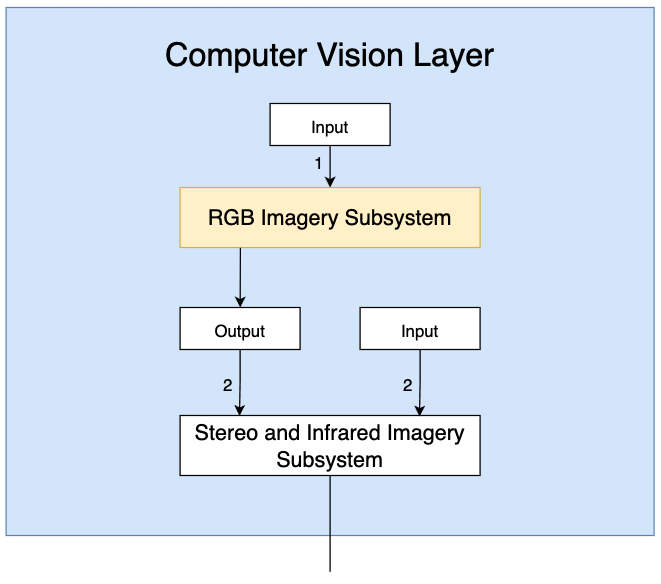
\includegraphics[width=0.70\textwidth]{images/CV_RGB.png}
 \caption{RGB Imagery subsystem description diagram}
\end{figure}

\subsubsection{Assumptions}
This layer is triggered by the user via the native iOS/Android application. It is assumed that the layer is being called upon in terrain with sufficient lighting conditions so that the RGB camera is able to produces images of good quality. For the \textit{Follow Me} feature, it is assumed that the user has their anklet put on and proceeds to start with the anklet within the frame of the camera. 

\subsubsection{Responsibilities}
RGB imagery is responsible for powering the \textit{Follow Along} and the \textit{Summon} features. For the \textit{Follow Along} feature, this subsystem calculates the position of the user in 1D space along the horizontal axis to determine whether to turn left, right, or straight. For the \textit{Summon} feature, this subsystem is responsible for helping identify patterns for possible obstacles ahead. 

\subsubsection{Subsystem Interfaces}
Each of the inputs and outputs for the subsystem are defined here. 

\begin {table}[H]
\caption {RGB Imagery Interfaces} 
\begin{center}
    \begin{tabular}{ | p{1cm} | p{6cm} | p{3cm} | p{3cm} |}
    \hline
    ID & Description & Inputs & Outputs \\ \hline
    1 & RGB Imagery & \pbox{3cm}{RGB Frame} & \pbox{3cm}{\phantom{Boo!}\\ Position of target object(s)\\}  \\ \hline
    \end{tabular}
\end{center}
\end{table}

\subsection{Stereo and Infrared Imagery Subsystem}
Stereo and Infrared Imagery of the front of the board is used as input in making various depth specific calculations pertaining to navigation.

\begin{figure}[h!]
	\centering
 	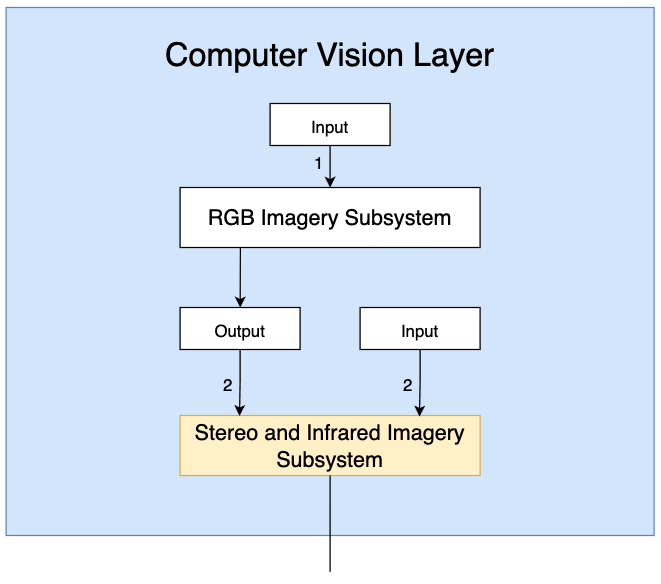
\includegraphics[width=0.70\textwidth]{images/CV_SIR.png}
 \caption{Stereo Imagery subsystem description diagram}
\end{figure}

\subsubsection{Assumptions}
This layer is triggered by the user via the native iOS/Android application. It is assumed that the layer is being called upon in terrain with sufficient lighting conditions so that the RGB Stereo cameras are able to produces images of good quality. For the \textit{Follow Me} feature, it is assumed that the user has their anklet put on and proceeds to start with the anklet within the frame of the cameras. 

\subsubsection{Responsibilities}
Stereo and Infrared imagery is responsible for powering the \textit{Follow Along} and the \textit{Summon} features. For the \textit{Follow Along} feature, this subsystem calculates the position of the user in 1D space along the longitudinal axis to determine whether to move forward or stay put. For the \textit{Summon} feature, this subsystem is responsible for helping identify how far objects detected by the RGB module are. 

\subsubsection{Subsystem Interfaces}
Each of the inputs and outputs for the subsystem are defined here.

\begin {table}[H]
\caption {Stereo and Infrared Imagery Interfaces} 
\begin{center}
    \begin{tabular}{ | p{1cm} | p{6cm} | p{3cm} | p{3cm} |}
    \hline
    ID & Description & Inputs & Outputs \\ \hline
    2 & Depth Imagery & \pbox{3cm}{Depth Frame \\ \\ Position of target object(s)} & \pbox{3cm}{\phantom{Boo!}\\ Optimized distance of target object(s) from camera\\ \\True position of target object(s) in 2D space\\}  \\ \hline
    \end{tabular}
\end{center}
\end{table}
